% This is "sig-alternate.tex" V2.1 April 2013
% This file should be compiled with V2.5 of "sig-alternate.cls" May 2012
%
% This example file demonstrates the use of the 'sig-alternate.cls'
% V2.5 LaTeX2e document class file. It is for those submitting
% articles to ACM Conference Proceedings WHO DO NOT WISH TO
% STRICTLY ADHERE TO THE SIGS (PUBS-BOARD-ENDORSED) STYLE.
% The 'sig-alternate.cls' file will produce a similar-looking,
% albeit, 'tighter' paper resulting in, invariably, fewer pages.
%
% ----------------------------------------------------------------------------------------------------------------
% This .tex file (and associated .cls V2.5) produces:
%       1) The Permission Statement
%       2) The Conference (location) Info information
%       3) The Copyright Line with ACM data
%       4) NO page numbers
%
% as against the acm_proc_article-sp.cls file which
% DOES NOT produce 1) thru' 3) above.
%
% Using 'sig-alternate.cls' you have control, however, from within
% the source .tex file, over both the CopyrightYear
% (defaulted to 200X) and the ACM Copyright Data
% (defaulted to X-XXXXX-XX-X/XX/XX).
% e.g.
% \CopyrightYear{2007} will cause 2007 to appear in the copyright line.
% \crdata{0-12345-67-8/90/12} will cause 0-12345-67-8/90/12 to appear in the copyright line.
%
% ---------------------------------------------------------------------------------------------------------------
% This .tex source is an example which *does* use
% the .bib file (from which the .bbl file % is produced).
% REMEMBER HOWEVER: After having produced the .bbl file,
% and prior to final submission, you *NEED* to 'insert'
% your .bbl file into your source .tex file so as to provide
% ONE 'self-contained' source file.
%
% ================= IF YOU HAVE QUESTIONS =======================
% Questions regarding the SIGS styles, SIGS policies and
% procedures, Conferences etc. should be sent to
% Adrienne Griscti (griscti@acm.org)
%
% Technical questions _only_ to
% Gerald Murray (murray@hq.acm.org)
% ===============================================================
%
% For tracking purposes - this is V2.0 - May 2012

\documentclass{sig-alternate-05-2015}




\usepackage{times}
\usepackage{CJKutf8}
\usepackage{mathrsfs}
\usepackage{textcomp}
\usepackage{verbatim}
\usepackage{amsmath}
\usepackage{amsfonts}
\usepackage{xspace}
\usepackage{xcolor}
\usepackage{url}
\usepackage{balance}
\usepackage{booktabs}
\usepackage{multirow}
\usepackage{rotating}
\usepackage{fancyvrb}
\usepackage{lastpage}
\usepackage{alltt}
\usepackage{etoolbox}
\usepackage{cleveref} % After hyperref, listings
\usepackage{fancyhdr}
\usepackage{listings}

\usepackage{caption}
\usepackage{subcaption}

\usepackage{tikz}
\usetikzlibrary{shapes,snakes}


\usepackage{amsmath}
\usepackage{amssymb}
\usepackage{wasysym}

%The given symbol or text (\text{mytext}) in a circle
%To be used always in math mode
\newcommand{\circlesign}[1]{ 
    \mathbin{
        \mathchoice
        {\buildcirclesign{\displaystyle}{#1}}
        {\buildcirclesign{\textstyle}{#1}}
        {\buildcirclesign{\scriptstyle}{#1}}
        {\buildcirclesign{\scriptscriptstyle}{#1}}
    } 
}


\newcommand\buildcirclesign[2]{%
    \begin{tikzpicture}[baseline=(X.base), inner sep=0, outer sep=0]
    \node[draw,circle] (X)  {\ensuremath{#1 #2}};
    \end{tikzpicture}%
}

\definecolor{lbcolor}{rgb}{0.9,0.9,0.9}
\lstset{
    tabsize=2,    
    language=C,
    basicstyle=\footnotesize\ttfamily,
    upquote=true,
    aboveskip={1.5\baselineskip},
    columns=fixed,
    extendedchars=false,
    showtabs=false,
    showspaces=false,
    showstringspaces=false,
    identifierstyle=\ttfamily,
    keywordstyle=\color[rgb]{0,0,1},
    commentstyle=\color[rgb]{0.026,0.112,0.095},
    stringstyle=\color[rgb]{0.627,0.126,0.941},
    numberstyle=\color[rgb]{0.205, 0.142, 0.73},
}


\usepackage{macro}
\newenvironment{CompactItemize}{\begin{itemize}}{\end{itemize}}
\def\code#1{{\texttt{#1}}}


\usepackage{colorhist}
 
\usepackage{minted}



\begin{document}

% Copyright
\setcopyright{acmcopyright}
%\setcopyright{acmlicensed}
%\setcopyright{rightsretained}
%\setcopyright{usgov}
%\setcopyright{usgovmixed}
%\setcopyright{cagov}
%\setcopyright{cagovmixed}


% DOI
\doi{XX.XXX/XXX_X}

% ISBN
\isbn{XX}

%Conference
\conferenceinfo{XXXXX}{XXXX, 2013, XX, XX, XXX}

\acmPrice{\$15.00}

%
% --- Author Metadata here ---
\conferenceinfo{XXXXX}{'XXXX', USA}
%\CopyrightYear{2007} % Allows default copyright year (20XX) to be over-ridden - IF NEED BE.
%\crdata{0-12345-67-8/90/01}  % Allows default copyright data (0-89791-88-6/97/05) to be over-ridden - IF NEED BE.
% --- End of Author Metadata ---

\title{Docker Container-based Scalable Partitioning for Apache Spark
Scale-Up Server Scalability}
%\subtitle{[Extended Abstract]
%\titlenote{A full version of this paper is available as
%\textit{Author's Guide to Preparing ACM SIG Proceedings Using
%\LaTeX$2_\epsilon$\ and BibTeX} at
%\texttt{www.acm.org/eaddress.htm}}}
%
% You need the command \numberofauthors to handle the 'placement
% and alignment' of the authors beneath the title.
%
% For aesthetic reasons, we recommend 'three authors at a time'
% i.e. three 'name/affiliation blocks' be placed beneath the title.
%
% NOTE: You are NOT restricted in how many 'rows' of
% "name/affiliations" may appear. We just ask that you restrict
% the number of 'columns' to three.
%
% Because of the available 'opening page real-estate'
% we ask you to refrain from putting more than six authors
% (two rows with three columns) beneath the article title.
% More than six makes the first-page appear very cluttered indeed.
%
% Use the \alignauthor commands to handle the names
% and affiliations for an 'aesthetic maximum' of six authors.
% Add names, affiliations, addresses for
% the seventh etc. author(s) as the argument for the
% \additionalauthors command.
% These 'additional authors' will be output/set for you
% without further effort on your part as the last section in
% the body of your article BEFORE References or any Appendices.



% Just remember to make sure that the TOTAL number of authors
% is the number that will appear on the first page PLUS the
% number that will appear in the \additionalauthors section.

\maketitle


%한글 버전으로 출력 하고 싶으면, korture를 Enable 해주시고, korefalse를 주석 처리 해주세요.
\newif\ifkor
\kortrue 
%\korfalse

\begin{abstract}
This paper provides a sample of a \LaTeX\ document which conforms,
somewhat loosely, to the formatting guidelines for
ACM SIG Proceedings. It is an {\em alternate} style which produces
a {\em tighter-looking} paper and was designed in response to
concerns expressed, by authors, over page-budgets.
It complements the document \textit{Author's (Alternate) Guide to
Preparing ACM SIG Proceedings Using \LaTeX$2_\epsilon$\ and Bib\TeX}.
This source file has been written with the intention of being
compiled under \LaTeX$2_\epsilon$\ and BibTeX.

\end{abstract}


%
% The code below should be generated by the tool at
% http://dl.acm.org/ccs.cfm
% Please copy and paste the code instead of the example below. 
%
\begin{CCSXML}
<ccs2012>
 <concept>
  <concept_id>10010520.10010553.10010562</concept_id>
  <concept_desc>Computer systems organization~Embedded systems</concept_desc>
  <concept_significance>500</concept_significance>
 </concept>
 <concept>
  <concept_id>10010520.10010575.10010755</concept_id>
  <concept_desc>Computer systems organization~Redundancy</concept_desc>
  <concept_significance>300</concept_significance>
 </concept>
 <concept>
  <concept_id>10010520.10010553.10010554</concept_id>
  <concept_desc>Computer systems organization~Robotics</concept_desc>
  <concept_significance>100</concept_significance>
 </concept>
 <concept>
  <concept_id>10003033.10003083.10003095</concept_id>
  <concept_desc>Networks~Network reliability</concept_desc>
  <concept_significance>100</concept_significance>
 </concept>
</ccs2012>  
\end{CCSXML}

\ccsdesc[500]{Computer systems organization~Embedded systems}
\ccsdesc[300]{Computer systems organization~Redundancy}
\ccsdesc{Computer systems organization~Robotics}
\ccsdesc[100]{Networks~Network reliability}


%
% End generated code
%

%
%  Use this command to print the description
%
\printccsdesc

% We no longer use \terms command
%\terms{Theory}

\keywords{ACM proceedings; \LaTeX; text tagging}

\def\bibfont{\footnotesize}


\ifkor
\begin{CJK}{UTF8}{}\CJKfamily{mj}
\fi
\section{Introduction} \label{sec:introduction}
%$$$$$$$$$$$$$$$$$$$$$$$$$$$$$$$$$$$$$$$$$$$$$$$$$$$$$$$$$$$$$$$$$$$$$$$$$$$$$$$$
%$$$$$$$$$$$$$$$$$$$$$$$$$$$$$$$$$$$$$$$$$$$$$$$$$$$$$$$$$$$$$$$$$$$$$$$$$$$$$$$$
%Background : 스파크 -> cloud가 아닌 single node에서의 scalability에 대한 연구가 필요해짐
%$$$$$$$$$$$$$$$$$$$$$$$$$$$$$$$$$$$$$$$$$$$$$$$$$$$$$$$$$$$$$$$$$$$$$$$$$$$$$$$$
\ifkor
빅데이터 처리하는데 중요한 방법 중 하나는 스파크이다.
스파크에 대한 연구는 그동안 
HPC를 위한 스파크가 필요하다. 
리눅스 운영체제가 많이 사용된다. 
기존 연구들은 scale-up 서버에 spark를 적용하기 위한 방법들[][]이 연구되고 있다.
하지만, 이러한 연구들은 리눅스 운영체제의 특징을 활용하지 못하는 문제점이 있다.
리눅스 운영체제 확장성에 대해서 가장 중요한것은 
리눅스는 conflit free한 운영체제가 아니다.
이유는~!!! 여러가지 상황을 고려하였기 때문에 
만약 응용프로그램이 scalalabe하게 디자인이 되어 있다면, 리눅스라도 스케일러블한 
상황으로 만들 수 있다~\cite{SilasBoydWickizer2010LinuxScales48}. 
\else

\fi

%$$$$$$$$$$$$$$$$$$$$$$$$$$$$$$$$$$$$$$$$$$$$$$$$$$$$$$$$$$$$$$$$$$$$$$$$$$$$$$$$
%$$$$$$$$$$$$$$$$$$$$$$$$$$$$$$$$$$$$$$$$$$$$$$$$$$$$$$$$$$$$$$$$$$$$$$$$$$$$$$$$
%Problem : NUMA 시스템으로 구성된 single node로 scalability가 없음 
% 2가지 관련 연구가 있음.
% 1. 24코어 이하의 서버에서의 Scalability 분석을 하였으나 해결책을 제안하지 않았음.
% 2. HPC(100이상) 으로 분석하였으나 flie system 관점으로 분석하였음.:메인 병목지점은 파일 시스템
% 3. Scalable한 파일 시스템을 사용한 후 Scalability에 대한 분석한 결과와 해결방법은 없음.
%$$$$$$$$$$$$$$$$$$$$$$$$$$$$$$$$$$$$$$$$$$$$$$$$$$$$$$$$$$$$$$$$$$$$$$$$$$$$$$$$
\ifkor
Scale-Up 서버를 위한 scalability 연구들이 진행되고 있다.
하지만, XX et al.은 scale-up 서버에서의 Scalability를 문제점을 구체적으로
분석하여 문제점을 보여주었으나, 해결책을 제안하지 않았다. 
XX et al.는 single note HPC에서의 문제점을 파일 시스템 관점으로 분석하였고, 
파일 시스템 관점으로 성능을 높혔다. 
하지만 아직 scalable한 파일 시스템을 사용해서 발생하는 spark의 scalability에 
문제점에 해결 방법은 아직 연구되지 않았다.
\else


\fi


%$$$$$$$$$$$$$$$$$$$$$$$$$$$$$$$$$$$$$$$$$$$$$$$$$$$$$$$$$$$$$$$$$$$$$$$$$$$$$$$$
%본 연구에서 분석한 결과와 제안하는 방법으로 향상된 성능
%$$$$$$$$$$$$$$$$$$$$$$$$$$$$$$$$$$$$$$$$$$$$$$$$$$$$$$$$$$$$$$$$$$$$$$$$$$$$$$$$
%$$$$$$$$$$$$$$$$$$$$$$$$$$$$$$$$$$$$$$$$$$$$$$$$$$$$$$$$$$$$$$$$$$$$$$$$$$$$$$$$
\ifkor
본 연구는 Scalable한 파일 시스템을 사용하여 파일 시스템에 대한 병목 지점을 
제거한 후 spark scalability를 분석을 하였고, 새로운 파티션닝 기법의 해결책을 제안한다. 
새로운 파티션닝 기법은 docker container를 이용하였고, 그 결과 shared-memory 시스템을 마치
distributed-system 처럼 구성하여 scalability를 향상 시켰다.
우리의 방법은 결국 Scale-up 서버의 NUMA 구조에 따른 memory access latency와 
shared-memory 시스템의 공유 때문에 발생하는 문제들(e.g, lock contention[], 
serialized garbage collect[],
single address space problem[], 
cache communication overhead[])를 해결한다.
\else


\fi



%$$$$$$$$$$$$$$$$$$$$$$$$$$$$$$$$$$$$$$$$$$$$$$$$$$$$$$$$$$$$$$$$$$$$$$$$$$$$$$$$
%본 연구에서 분석한 결과와 제안하는 방법으로 향상된 성능
%$$$$$$$$$$$$$$$$$$$$$$$$$$$$$$$$$$$$$$$$$$$$$$$$$$$$$$$$$$$$$$$$$$$$$$$$$$$$$$$$
%$$$$$$$$$$$$$$$$$$$$$$$$$$$$$$$$$$$$$$$$$$$$$$$$$$$$$$$$$$$$$$$$$$$$$$$$$$$$$$$$
\ifkor
Scalability 문제를 해결하기 위해, 본 연구는 메모리 파티션 기반의 JailDocker를 만들었다. 
JailDocker는 Scale-Up server에서 최적의 성능을 내기 위한 파티션 방법이다. 
기반을 사용하기 우리는 Docker를 사용하였다. 
BigDataBench의 Wordcount on 120core.

\else


\fi

%$$$$$$$$$$$$$$$$$$$$$$$$$$$$$$$$$$$$$$$$$$$$$$$$$$$$$$$$$$$$$$$$$$$$$$$$$$$$$$$$
%본 연구에서 기여한 것 : 
% 1. 100코어 이상의 scale-up 서버에서의 scalability 측정 및 분석
% 2. 도커 파티션 기법을 활용한 scalability 향상 방법 제안
%$$$$$$$$$$$$$$$$$$$$$$$$$$$$$$$$$$$$$$$$$$$$$$$$$$$$$$$$$$$$$$$$$$$$$$$$$$$$$$$$
\ifkor

\textbf{Contributions.} Our research makes the following contributions:
\begin{itemize}
\item We have developed a novel lightweight log-based deferred update method
eliminating the sources of limiting performance scalability in update-heavy data
structures with efficient log management implementation.
\item 
We applied the in Linux kernel to two reverse mapping(anonymous, file) on
an 120 core system to reduce fork scalability bottleneck.
Our design improved throughput and execution time from 1.5x through 2.7x on 120 core.
\end{itemize}

\else

\fi


%$$$$$$$$$$$$$$$$$$$$$$$$$$$$$$$$$$$$$$$$$$$$$$$$$$$$$$$$$$$$$$$$$$$$$$$$$$$$$$$$
%$$$$$$$$$$$$$$$$$$$$$$$$$$$$$$$$$$$$$$$$$$$$$$$$$$$$$$$$$$$$$$$$$$$$$$$$$$$$$$$$
%Mapping
%$$$$$$$$$$$$$$$$$$$$$$$$$$$$$$$$$$$$$$$$$$$$$$$$$$$$$$$$$$$$$$$$$$$$$$$$$$$$$$$$
The rest of this paper is organized as follows.
Section 2 describes the background and the Linux scalability problem.
Section 3 describes the design of the algorithm and 
Section 4 explains how to apply the to Linux kernel, and
Section 5 shows the results of the experimental evaluation. 
Finally, section 6 concludes the paper.




\section{Scale-up Server Scalalbility}




%$$$$$$$$$$$$$$$$$$$$$$$$$$$$$$$$$$$$$$$$$$$$$$$$$$$$$$$$$$$$$$$$$$$$$$$$$$$$$$$$
%$$$$$$$$$$$$$$$$$$$$$$$$$$$$$$$$$$$$$$$$$$$$$$$$$$$$$$$$$$$$$$$$$$$$$$$$$$$$$$$$
% 이번 장에 대한 설명
%$$$$$$$$$$$$$$$$$$$$$$$$$$$$$$$$$$$$$$$$$$$$$$$$$$$$$$$$$$$$$$$$$$$$$$$$$$$$$$$$
\ifkor
\else

\fi



\subsection{Test-bed and Benchmark}

%$$$$$$$$$$$$$$$$$$$$$$$$$$$$$$$$$$$$$$$$$$$$$$$$$$$$$$$$$$$$$$$$$$$$$$$$$$$$$$$$
%$$$$$$$$$$$$$$$$$$$$$$$$$$$$$$$$$$$$$$$$$$$$$$$$$$$$$$$$$$$$$$$$$$$$$$$$$$$$$$$$
% Apache Spark에 대한 설명
%$$$$$$$$$$$$$$$$$$$$$$$$$$$$$$$$$$$$$$$$$$$$$$$$$$$$$$$$$$$$$$$$$$$$$$$$$$$$$$$$
\ifkor
\noindent
\textbf{Apache Spark. }
Apache Spark is a framework for large scale distributed computation.
RDD(Resilient Distributed Datasets) is a collection of partitions of records, 
and the RDD is managed as LRU(Least Recently Used), so when there is not enough
memory, Spark evits the least recently used RDD.
Spark may has a substantial performance when dataset can fit in memory.

%\begin{figure}[h]
%    \centering
%    \begin{subfigure}[b]{0.22\textwidth}
%        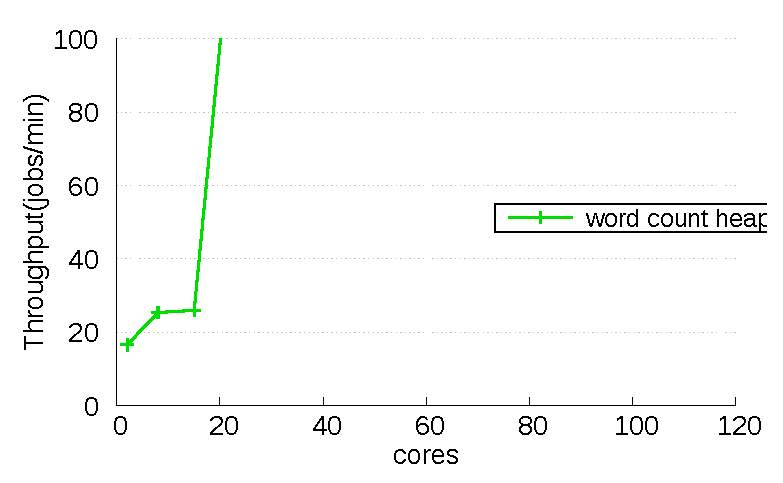
\includegraphics[width=1.5in]{graph/wc_max.eps}
%        \caption{Word Count}
%    \end{subfigure}%
%    \begin{subfigure}[b]{0.22\textwidth}
%        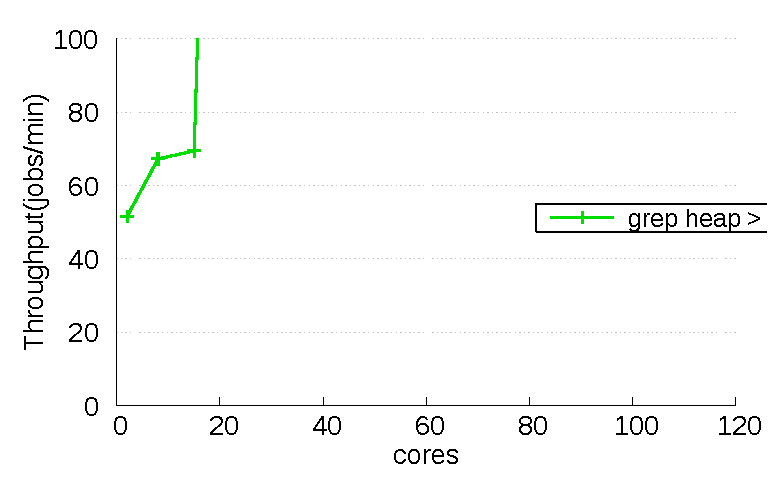
\includegraphics[width=1.5in]{graph/grep_max.eps}
%        \caption{Grep}
%    \end{subfigure}
%    \caption{CPU utilization on 120 core.}
%    \label{fig:utilization}
%\end{figure}

%Figure shows a substantial performance scalability of Spark when dataset can
% fit in memory(heap size > data size).
%However, large scale data(head size < data size) does not scale on scale-up
%server due to the GC and the memory latency.
\else
\fi

%$$$$$$$$$$$$$$$$$$$$$$$$$$$$$$$$$$$$$$$$$$$$$$$$$$$$$$$$$$$$$$$$$$$$$$$$$$$$$$$$
%$$$$$$$$$$$$$$$$$$$$$$$$$$$$$$$$$$$$$$$$$$$$$$$$$$$$$$$$$$$$$$$$$$$$$$$$$$$$$$$$
% 테스트 베드 설명
%$$$$$$$$$$$$$$$$$$$$$$$$$$$$$$$$$$$$$$$$$$$$$$$$$$$$$$$$$$$$$$$$$$$$$$$$$$$$$$$$
\ifkor
\noindent
\textbf{Test-bed. }
We use a machine to evaluate on real hardware: an 120-core (8 sockets × 15
cores) Intel Xeon E7-8870 (the same machine used for evaluation in chapter X)
and, to show that our conclusions generalize.
Hyper-Threading is disabled, and we used Linux kernel 4.5-rc6.

\begin{figure}[h]
  \begin{center}
     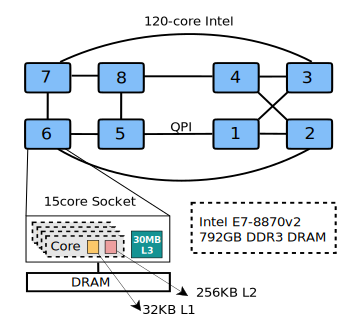
\includegraphics[width=0.3\textwidth]{fig/xeon}
  \end{center}
  \caption{Test-bed intel xeon archtecture.}
  \label{fig:basic}
\end{figure}
\else

\fi

%$$$$$$$$$$$$$$$$$$$$$$$$$$$$$$$$$$$$$$$$$$$$$$$$$$$$$$$$$$$$$$$$$$$$$$$$$$$$$$$$
%$$$$$$$$$$$$$$$$$$$$$$$$$$$$$$$$$$$$$$$$$$$$$$$$$$$$$$$$$$$$$$$$$$$$$$$$$$$$$$$$
%Benchamrk에 대한 설명
%$$$$$$$$$$$$$$$$$$$$$$$$$$$$$$$$$$$$$$$$$$$$$$$$$$$$$$$$$$$$$$$$$$$$$$$$$$$$$$$$
\ifkor
\noindent
\textbf{Benchmark.} We used BigData Benchmark.
\begin{itemize}
\item \textbf{Word Count. }We have developed a novel lightweight log-based
structures with efficient log management implementation.
\item \textbf{Grep. }
We applied the in Linux kernel to two reverse mapping(anonymous, file) on
Our design improved throughput and execution time from 1.5x through 2.7x on 120 core.
\item \textbf{Naive Basian. }
We applied the in Linux kernel to two reverse mapping(anonymous, file) on
Our design improved throughput and execution time from 1.5x through 2.7x on 120 core.
\item \textbf{K-means.}
We applied the in Linux kernel to two reverse mapping(anonymous, file) on
Our design improved throughput and execution time from 1.5x through 2.7x on 120 core.
\end{itemize}
\else

\fi


\subsection{Spark Scalability Problem}
%$$$$$$$$$$$$$$$$$$$$$$$$$$$$$$$$$$$$$$$$$$$$$$$$$$$$$$$$$$$$$$$$$$$$$$$$$$$$$$$$
%$$$$$$$$$$$$$$$$$$$$$$$$$$$$$$$$$$$$$$$$$$$$$$$$$$$$$$$$$$$$$$$$$$$$$$$$$$$$$$$$
%Scalability 결과에 대한 대략 적인 설명
%$$$$$$$$$$$$$$$$$$$$$$$$$$$$$$$$$$$$$$$$$$$$$$$$$$$$$$$$$$$$$$$$$$$$$$$$$$$$$$$$
\ifkor
Figure 1 shows the spark scalability of five workloads with G1 and Parallel
Scavenge GC(PS).
Up to 60 core, The five workloads scales linealy and then GC pause become
bottlenecks.
The word count flattens out after 60 core, but other benchmarks slightly go
down because not only GC overhead but also NUMA effects. 
To evalute state of the art GC, we used G1 and PS GC.
The result of impact of chainging the GC are PS GC results in 3.3x better
performance than G1 GC on 120 core.
However, although we used the scalable GC, the Spark performance scalabiliy is
still limited by GC and NUMA effects.
\else

\fi


%$$$$$$$$$$$$$$$$$$$$$$$$$$$$$$$$$$$$$$$$$$$$$$$$$$$$$$$$$$$$$$$$$$$$$$$$$$$$$$$$
%$$$$$$$$$$$$$$$$$$$$$$$$$$$$$$$$$$$$$$$$$$$$$$$$$$$$$$$$$$$$$$$$$$$$$$$$$$$$$$$$
%CPU utilization에 대한 설명
%$$$$$$$$$$$$$$$$$$$$$$$$$$$$$$$$$$$$$$$$$$$$$$$$$$$$$$$$$$$$$$$$$$$$$$$$$$$$$$$$

\ifkor
Figure ~\ref{fig:cpuutilization} shows the job's CPU utilization.
Our goal is high cpu utilization, 
Th y-axis is the percentage of time spent in kernel-space code(sys), user-space
code(user), and idle time(idle).
When core counts increase, all benchmarks increase idle time due to GC pasue
that means 

\else

\fi


%$$$$$$$$$$$$$$$$$$$$$$$$$$$$$$$$$$$$$$$$$$$$$$$$$$$$$$$$$$$$$$$$$$$$$$$$$$$$$$$$
%$$$$$$$$$$$$$$$$$$$$$$$$$$$$$$$$$$$$$$$$$$$$$$$$$$$$$$$$$$$$$$$$$$$$$$$$$$$$$$$$
% Linux kernel scalability (lock, cache cohearnci, scheduler)등등 OS 노이즈에 대한 설명
%$$$$$$$$$$$$$$$$$$$$$$$$$$$$$$$$$$$$$$$$$$$$$$$$$$$$$$$$$$$$$$$$$$$$$$$$$$$$$$$$
\ifkor
%NUMA의 영향 뿐만 아니라, 추가적으로 operating system의 scalability 저해 요소 때문에 
%파티션닝 방법은 필요하다.
%우리는 operation system에서 scalability의 영향을 주는 것을 확인하기 위해 가장먼저
%lock을 조사해보았다.
%첫째로 공유 데이터를 lock이 있다. 표 xxx 앞에서 실험한 spark의 wordcount에 대해서 .
%JVM 위에서 동작하는 thread간의 공유하는 single address space때문에 발생하는 공유 문제이다.
%다음으로 scheduler가 아직 
%마지막으로 cache cohearci traffic이 있다. 
\else

\fi



\subsection{Benefit of JVM Partitioning}
%\subsection{NUMA}

%$$$$$$$$$$$$$$$$$$$$$$$$$$$$$$$$$$$$$$$$$$$$$$$$$$$$$$$$$$$$$$$$$$$$$$$$$$$$$$$$
%$$$$$$$$$$$$$$$$$$$$$$$$$$$$$$$$$$$$$$$$$$$$$$$$$$$$$$$$$$$$$$$$$$$$$$$$$$$$$$$$
%NUMA 영향에 대한 대략 적인 설명
%$$$$$$$$$$$$$$$$$$$$$$$$$$$$$$$$$$$$$$$$$$$$$$$$$$$$$$$$$$$$$$$$$$$$$$$$$$$$$$$$

\ifkor
Spark and Hadoop ramework use JAVA and it needs java virtual machine, so
understanding the partitioning effect on JVM is importance.
To preliminarily analysis the JVM partitioning effect, we conducted
benchamrking by using SPECjbb2013~\cite{PPogue2014SO}, which a state of the art
benchmark for JVM performance.
We used two different experiment settings. First, we used per-socket
JVM partitioning using the numa control application(numactl).
Second, we set maxium available memory to JVM heap size and
threads are scheduled by the OS in order to migrate any core, and we
enable automatic NUMA balancing feature in the Linux kernel.
\else
\fi

\begin{figure}[h]
  \begin{center}
     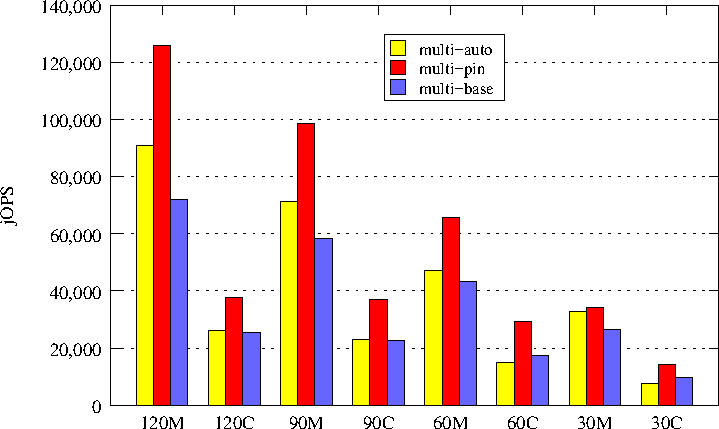
\includegraphics[width=0.4\textwidth]{graph/SPECjbb2013}
  \end{center}
  \caption{Test-bed Intel xeon archtecture.}
  \label{fig:basic}
\end{figure}

\ifkor

The results all core shows that partitioning approach outperforms than
non-partitioning approach by Xx on 120 core.
In manycore scale-up server, partiting approach has best performance
scalability.
\else
\fi

\section{Scalable Partitioning}
%$$$$$$$$$$$$$$$$$$$$$$$$$$$$$$$$$$$$$$$$$$$$$$$$$$$$$$$$$$$$$$$$$$$$$$$$$$$$$$$$
%$$$$$$$$$$$$$$$$$$$$$$$$$$$$$$$$$$$$$$$$$$$$$$$$$$$$$$$$$$$$$$$$$$$$$$$$$$$$$$$$
% 이번 장에 대한 설명
%$$$$$$$$$$$$$$$$$$$$$$$$$$$$$$$$$$$$$$$$$$$$$$$$$$$$$$$$$$$$$$$$$$$$$$$$$$$$$$$$
\ifkor
이번 장에서는 스파크의 Scalalbility에 대해서 설명한다.
\else

\fi

%$$$$$$$$$$$$$$$$$$$$$$$$$$$$$$$$$$$$$$$$$$$$$$$$$$$$$$$$$$$$$$$$$$$$$$$$$$$$$$$$
%$$$$$$$$$$$$$$$$$$$$$$$$$$$$$$$$$$$$$$$$$$$$$$$$$$$$$$$$$$$$$$$$$$$$$$$$$$$$$$$$
% 일반적인 매니코어 또는 Scale-server Partitioning에 대한 설명 
%$$$$$$$$$$$$$$$$$$$$$$$$$$$$$$$$$$$$$$$$$$$$$$$$$$$$$$$$$$$$$$$$$$$$$$$$$$$$$$$$
\ifkor
이번 장에서는 스파크의 Scalalbility에 대해서 설명한다.
\else

\fi

%$$$$$$$$$$$$$$$$$$$$$$$$$$$$$$$$$$$$$$$$$$$$$$$$$$$$$$$$$$$$$$$$$$$$$$$$$$$$$$$$
%$$$$$$$$$$$$$$$$$$$$$$$$$$$$$$$$$$$$$$$$$$$$$$$$$$$$$$$$$$$$$$$$$$$$$$$$$$$$$$$$
% NUMA 영향에 대한 설명
%$$$$$$$$$$$$$$$$$$$$$$$$$$$$$$$$$$$$$$$$$$$$$$$$$$$$$$$$$$$$$$$$$$$$$$$$$$$$$$$$
\ifkor
이번 장에서는 스파크의 Scalalbility에 대해서 설명한다.
\else

\fi


%$$$$$$$$$$$$$$$$$$$$$$$$$$$$$$$$$$$$$$$$$$$$$$$$$$$$$$$$$$$$$$$$$$$$$$$$$$$$$$$$
%$$$$$$$$$$$$$$$$$$$$$$$$$$$$$$$$$$$$$$$$$$$$$$$$$$$$$$$$$$$$$$$$$$$$$$$$$$$$$$$$
% Linux kernel scalability (lock, cache cohearnci, scheduler)등등 OS 노이즈에 대한 설명
%$$$$$$$$$$$$$$$$$$$$$$$$$$$$$$$$$$$$$$$$$$$$$$$$$$$$$$$$$$$$$$$$$$$$$$$$$$$$$$$$
\ifkor
이번 장에서는 스파크의 Scalalbility에 대해서 설명한다.
\else

\fi

%$$$$$$$$$$$$$$$$$$$$$$$$$$$$$$$$$$$$$$$$$$$$$$$$$$$$$$$$$$$$$$$$$$$$$$$$$$$$$$$$
%$$$$$$$$$$$$$$$$$$$$$$$$$$$$$$$$$$$$$$$$$$$$$$$$$$$$$$$$$$$$$$$$$$$$$$$$$$$$$$$$
% 스파크는 결국 : shared memory system -> distributed system 처럼해야한다. 
%$$$$$$$$$$$$$$$$$$$$$$$$$$$$$$$$$$$$$$$$$$$$$$$$$$$$$$$$$$$$$$$$$$$$$$$$$$$$$$$$
\ifkor
이번 장에서는 스파크의 Scalalbility에 대해서 설명한다.
\else

\fi



%$$$$$$$$$$$$$$$$$$$$$$$$$$$$$$$$$$$$$$$$$$$$$$$$$$$$$$$$$$$$$$$$$$$$$$$$$$$$$$$$
%$$$$$$$$$$$$$$$$$$$$$$$$$$$$$$$$$$$$$$$$$$$$$$$$$$$$$$$$$$$$$$$$$$$$$$$$$$$$$$$$
% 제안하는 구조 framework 설명
%$$$$$$$$$$$$$$$$$$$$$$$$$$$$$$$$$$$$$$$$$$$$$$$$$$$$$$$$$$$$$$$$$$$$$$$$$$$$$$$$
\ifkor
이번 장에서는 스파크의 Scalalbility에 대해서 설명한다.
\else

\fi





%$$$$$$$$$$$$$$$$$$$$$$$$$$$$$$$$$$$$$$$$$$$$$$$$$$$$$$$$$$$$$$$$$$$$$$$$$$$$$$$$
%$$$$$$$$$$$$$$$$$$$$$$$$$$$$$$$$$$$$$$$$$$$$$$$$$$$$$$$$$$$$$$$$$$$$$$$$$$$$$$$$
% Docker를 이용하는 이유
%$$$$$$$$$$$$$$$$$$$$$$$$$$$$$$$$$$$$$$$$$$$$$$$$$$$$$$$$$$$$$$$$$$$$$$$$$$$$$$$$
\ifkor
이번 장에서는 스파크의 Scalalbility에 대해서 설명한다.
\else

\fi



%$$$$$$$$$$$$$$$$$$$$$$$$$$$$$$$$$$$$$$$$$$$$$$$$$$$$$$$$$$$$$$$$$$$$$$$$$$$$$$$$
%$$$$$$$$$$$$$$$$$$$$$$$$$$$$$$$$$$$$$$$$$$$$$$$$$$$$$$$$$$$$$$$$$$$$$$$$$$$$$$$$
% 알고리즘 
%$$$$$$$$$$$$$$$$$$$$$$$$$$$$$$$$$$$$$$$$$$$$$$$$$$$$$$$$$$$$$$$$$$$$$$$$$$$$$$$$
\ifkor
이번 장에서는 스파크의 Scalalbility에 대해서 설명한다.
\else

\fi



\section{Evaluation}


\begin{figure*}[tb]
    \centering
    \begin{subfigure}[b]{0.25\textwidth}
        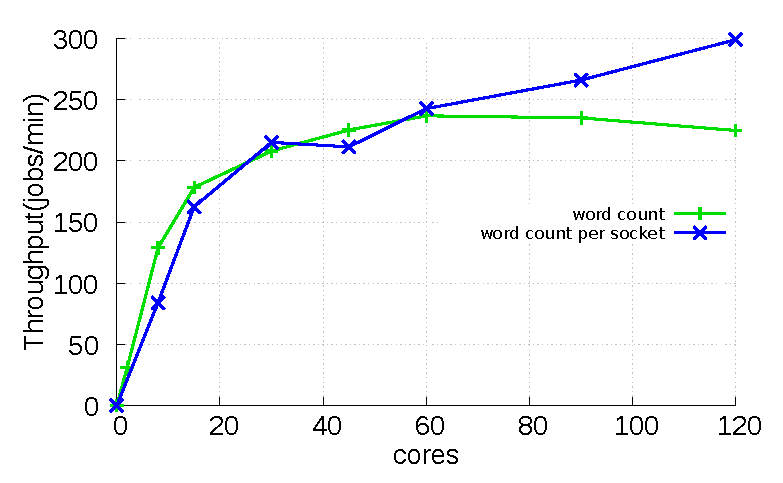
\includegraphics[width=1.8in]{graph/wc_docker.eps}
        \caption{Exim - 120core}
    \end{subfigure}%
    \begin{subfigure}[b]{0.25\textwidth}
        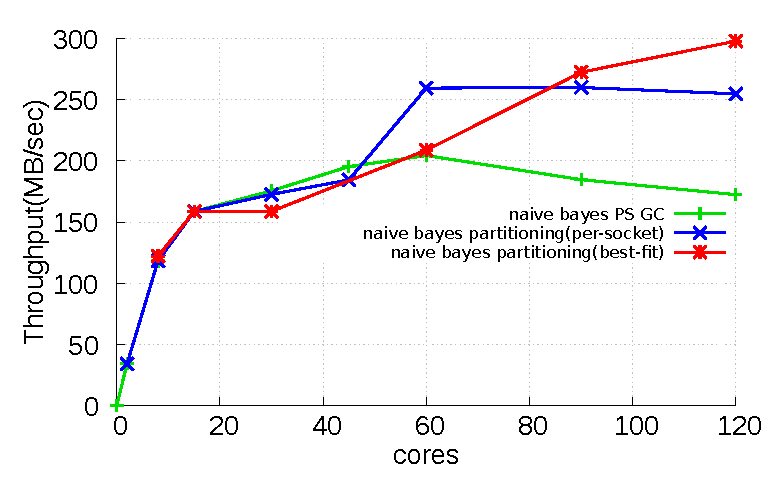
\includegraphics[width=1.8in]{graph/nb_docker.eps}
        \caption{Lmbench - 120core}
    \end{subfigure}%
    \begin{subfigure}[b]{0.25\textwidth}
        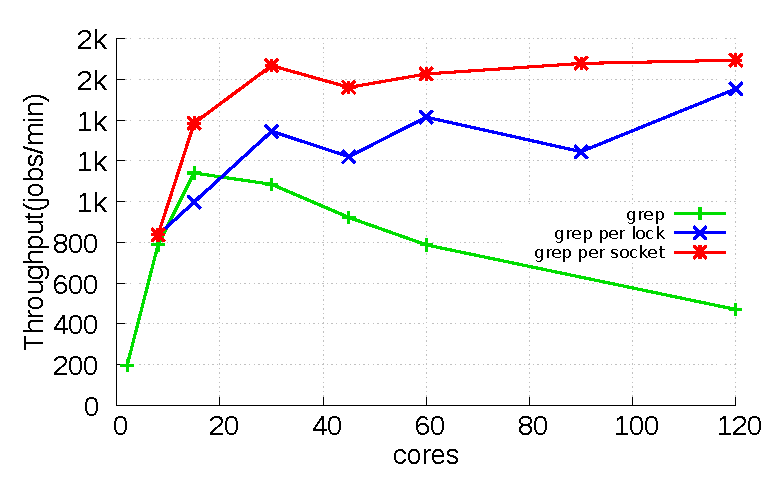
\includegraphics[width=1.8in]{graph/grep_docker.eps}
        \caption{AIM7 - 120core}
    \end{subfigure}%
        \begin{subfigure}[b]{0.25\textwidth}
        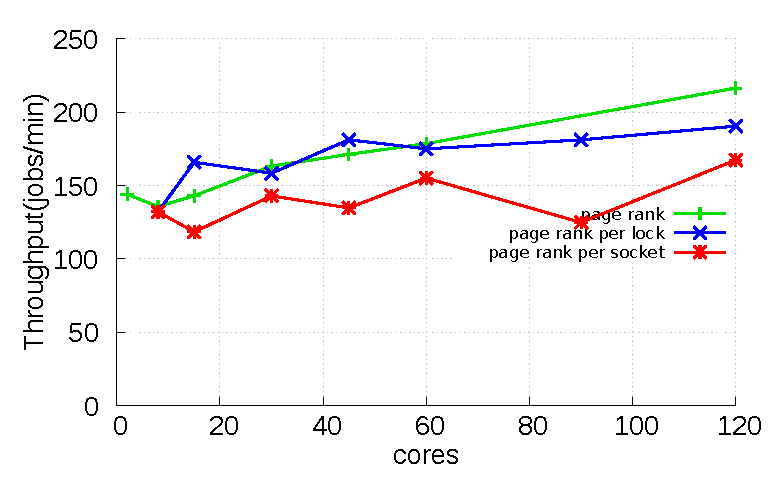
\includegraphics[width=1.8in]{graph/pagerank_docker.eps}
        \caption{Lmbench - 120core}
    \end{subfigure}
        \centering
    \caption{CPU utilization on 120 core.}
    \label{fig:utilization3}
\end{figure*}



\begin{figure*}[tb]
    \centering
    \begin{subfigure}[b]{0.25\textwidth}
        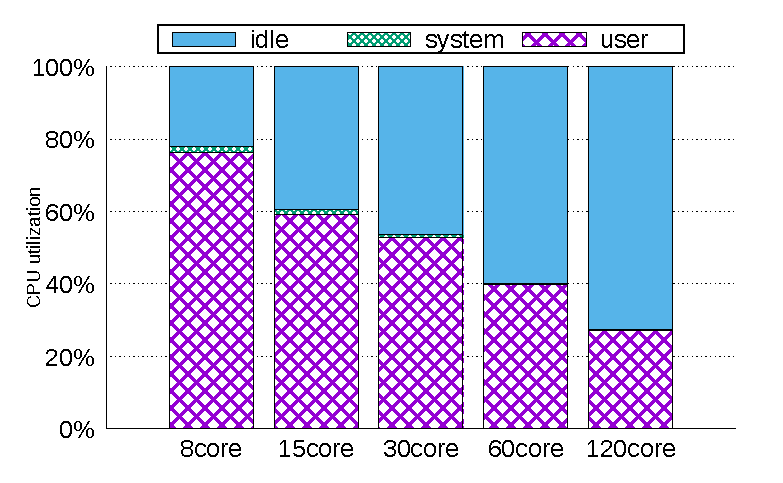
\includegraphics[width=1.8in]{graph/wc_cpuutils.eps}
        \caption{Word Count}
    \end{subfigure}%
    \begin{subfigure}[b]{0.25\textwidth}
        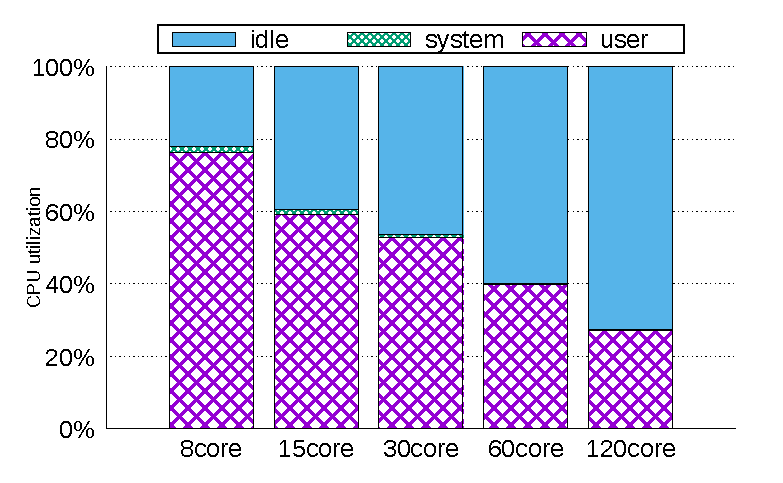
\includegraphics[width=1.8in]{graph/wc_cpuutils.eps}
        \caption{Naive Basian}
    \end{subfigure}%
    \begin{subfigure}[b]{0.25\textwidth}
        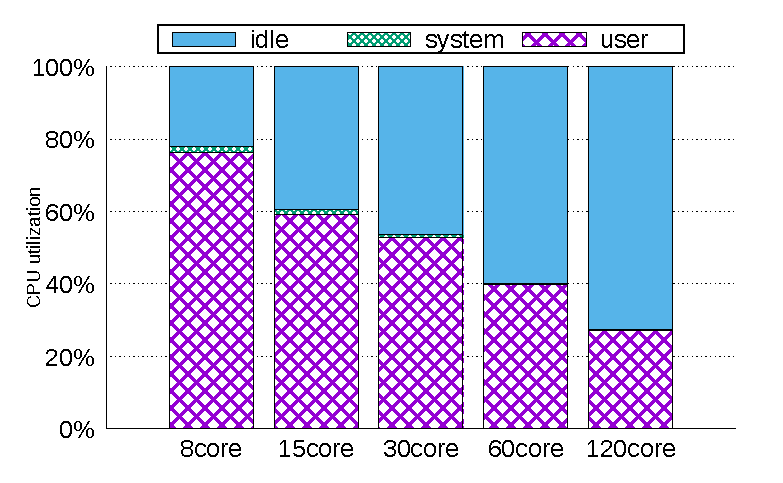
\includegraphics[width=1.8in]{graph/wc_cpuutils.eps}
        \caption{Grep}
    \end{subfigure}%
        \begin{subfigure}[b]{0.25\textwidth}
        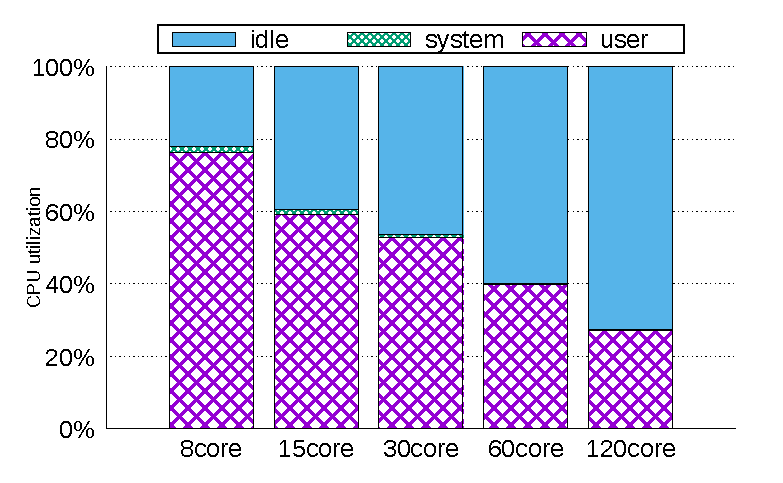
\includegraphics[width=1.8in]{graph/wc_cpuutils.eps}
        \caption{Pagerank}
    \end{subfigure}
        \centering
    \caption{CPU utilization on 120 core.}
    \label{fig:utilization2}
\end{figure*}




%$$$$$$$$$$$$$$$$$$$$$$$$$$$$$$$$$$$$$$$$$$$$$$$$$$$$$$$$$$$$$$$$$$$$$$$$$$$$$$$$
%Paragraph 1: 무엇을 평가 했는지에 대한 설명 
%$$$$$$$$$$$$$$$$$$$$$$$$$$$$$$$$$$$$$$$$$$$$$$$$$$$$$$$$$$$$$$$$$$$$$$$$$$$$$$$$

This section answers the following questions experimentally:
\begin{CompactItemize}
\item Does \ldu's design matter for applications?

\item Why does \ldu's scheme scale well?

\item What about \ldu's read-write ratio?
\end{CompactItemize}


\section{Related work} \label{sec:RelatedWork}

%$$$$$$$$$$$$$$$$$$$$$$$$$$$$$$$$$$$$$$$$$$$$$$$$$$$$$$$$$$$$$$$$$$$$$$$$$$$$$$$$
%Paragraph 1:Linux Scalability의 연구에 대한 설명
%$$$$$$$$$$$$$$$$$$$$$$$$$$$$$$$$$$$$$$$$$$$$$$$$$$$$$$$$$$$$$$$$$$$$$$$$$$$$$$$$
\noindent 
\textbf{Apache Spark Scalability.}
To improve the Spark scalability, researchers have attempted to optimize for
scale-out server~\cite{Ousterhout2015MSP}~\cite{Maas2016THL} or to optimize scale-up server~\cite{Ahsan2016SVS}~\cite{Chaimov2016SSH}.
Our research belongs to optimizing for scale-up server to eliminate GC overheads
and to enhance the locality on NUMA architecture.
However, previous studies did not considered Docker container-based partitioning,
which can clearly reduce memory contention, and it can maximize locality of memory access.
Furthermore, it can easily combine other container management solutions.

%$$$$$$$$$$$$$$$$$$$$$$$$$$$$$$$$$$$$$$$$$$$$$$$$$$$$$$$$$$$$$$$$$$$$$$$$$$$$$$$$
%Paragraph 1:Manycore Scalability의 연구에 대한 설명
%$$$$$$$$$$$$$$$$$$$$$$$$$$$$$$$$$$$$$$$$$$$$$$$$$$$$$$$$$$$$$$$$$$$$$$$$$$$$$$$$
\noindent
\textbf{Scale-up Server Scalability.}
To improve the Spark scalability, researchers have attempted to apply distributed
system concepts to shared
memory systems~\cite{Baumann2009Barrelfish}~\cite{SilasBoydWickizerPth}.
Barrelfish~\cite{Baumann2009Barrelfish} creates a new operating system for efficient cache-coherent
shared memory system by building an OS using message-based architecture.
Our research also brings about distributed system concepts, but our approach applies
to user level Spark framework instead of OS because OS can achieves 
performance scalability by commuting interface~\cite{Clements2013SCR}.

\section{Conclusion}
\ifkor
\else

\fi


\bibliographystyle{plain}
\bibliography{ref}

\ifkor
\end{CJK}
\fi

% That's all folks!
\end{document}
